\dev{Emile Martinez}{Balabonski MPI}

\textit{Ce développement présente la création et la recherche dans des arbres K-dimensionnels. Il s'insère donc dans la leçon sur les arbres, sur les algorithmes d'apprentissage (pour k-PPV) et dans la leçon diviser pour régner en insistant plus sur les notions de ce paradigme de ce développement.}

\paragraph{Objectif :} Prétraiter n points de $\mathbb R^K$ pour que l'on puisse rapidement trouver les $k$ plus proches voisins d'un point $x\in \mathbb R^K$

\section*{Construction}

\paragraph{Idée :} 
Un arbre $K$-dimensionnel de $n$ points de $\mathbb R^K$ est un arbre binaire de recherche sur $K$ dimension :
\begin{itemize}[label=$\star$]
	\item chaque noeud contient un point
	\item pour un noeud à la profondeur $i$ contenant le point $x$,\begin{itemize}[label=$\bullet$]
		\item pour y contenu dans le sous arbre gauche de $x$, $y_{i\%K} \leq x_{i\%K}$
		\item pour y contenu dans le sous arbre droit de $x$, $y_{i\%K} \geq x_{i\%K}$
	\end{itemize}
	\item les sous arbres gauche et droit d'un noeud ont a peu près la même taille.
\end{itemize}

\paragraph{construction :} Si on est à la profondeur $i$ :
\begin{itemize}
	\item On prend la médiane selon la $i\%K$-ème coordonnée
	\item On construit l' arbres enraciné à la profondeur $i+1$ des points de $i\%K$-ième coordonnée inférieur (resp. supérieur) à la médiane qui deviendra le sous arbre gauche (resp. droit) de notre médiane
\end{itemize}

\paragraph{Exemple en deux dimensions} :\\
\raisebox{-0.5\height}{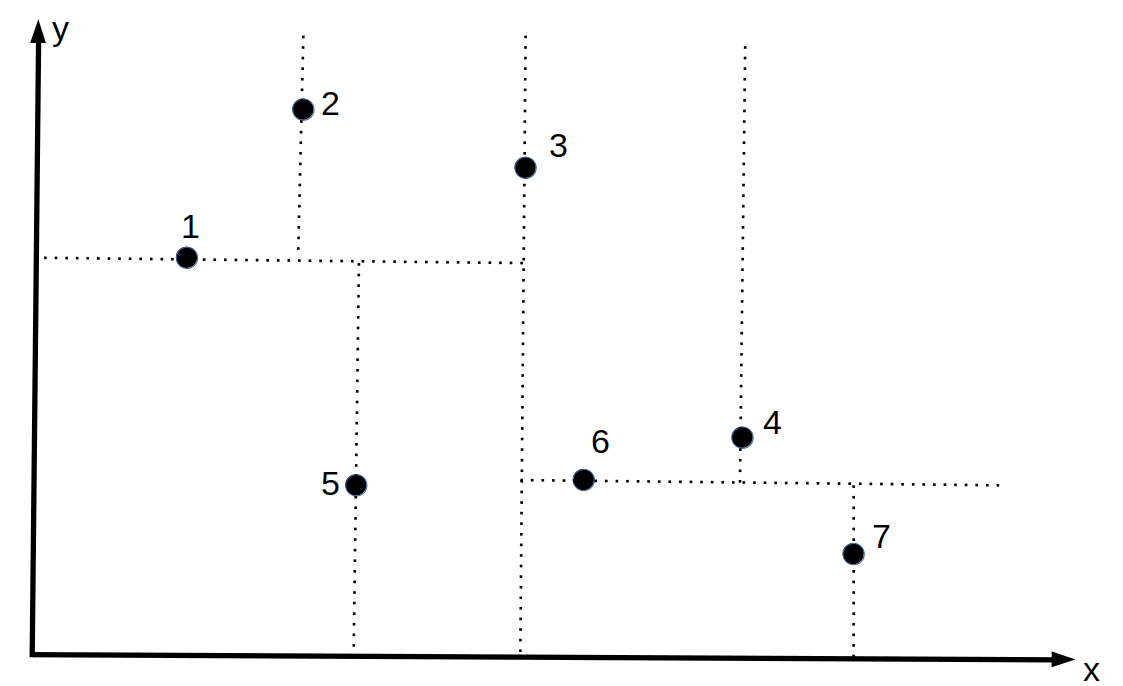
\includegraphics[height=6cm]{Developpements/arbre kdim/n_points.png}}
\raisebox{-0.5\height}{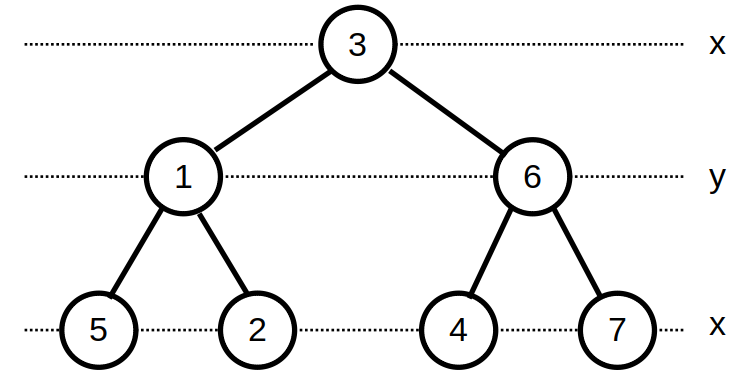
\includegraphics[height=4cm]{Developpements/arbre kdim/arbre.png}}

\section*{Recherche de k plus proche voisins}

\paragraph{Idée :} On cherche de préférence là où on aurait mis notre noeud
\begin{itemize}[label=$\star$]
	\item On cherche les $k$ plus proches voisins dans le sous arbre où notre noeud aurait était inséré
	\item Si les $k$ que l'on a trouvé sont suffisament loin pour que les plus proches puissent être dans un autre sous arbres, on remonte d'un cran et on cherche dans l'autre sous arbre, etc...	
\end{itemize}

\paragraph{Algorithme} Quand on cherche les voisins de $p$ à la hauteur $i$
\begin{enumerate}
	\item Si on a moins de $K$ noeuds dans notre sous arbre, on les renvoie et on complète avec des noeuds à distance $\infty$
	\item Sinon, on compare $p_{i\%K}$ à $x_{i\%K}$ où $x$ est le point de notre noeud. Si c'est inférieur, on cherche dans le sous arbre gauche, sinon dans le droit
	\item Quand on a récupérer $p1, \dots, pk$ nos $k$ voisins, on regarde si $x$ est plus proche. Si oui, on l'ajoute
	\item Notons $r$ la distance au point le plus éloigné. Si $r > c = \left|p_{i\%K} - x_{i\%K}\right|$, on cherche dans l'autre sous arbre et on garde les $k$ plus proches voisins des deux sous arbres.
	\item On renvoie les voisins que l'on a. 
\end{enumerate}

\paragraph{Illustration} Pour $K = 2$, un exemple du test de l'étape 4.\\
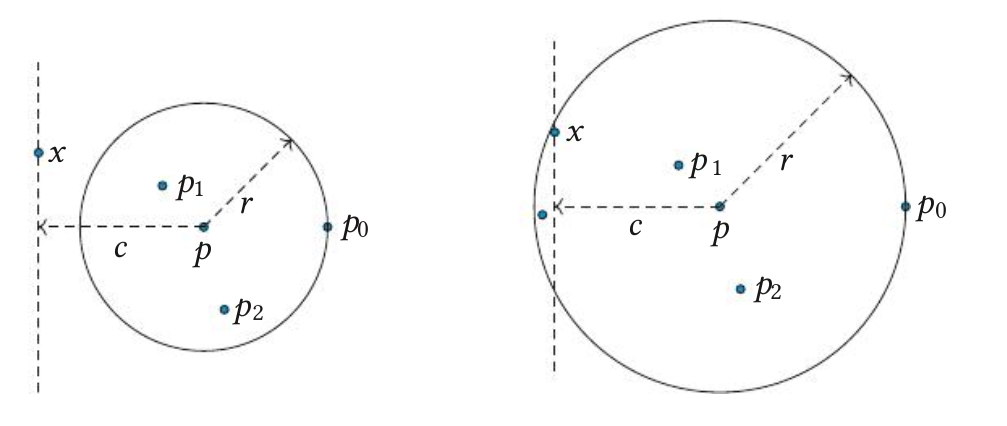
\includegraphics[scale = 0.4]{Developpements/arbre kdim/exemple_echec.png}

\paragraph{Exemple} Sur l'exemple de la construction : \\
\raisebox{-0.5\height}{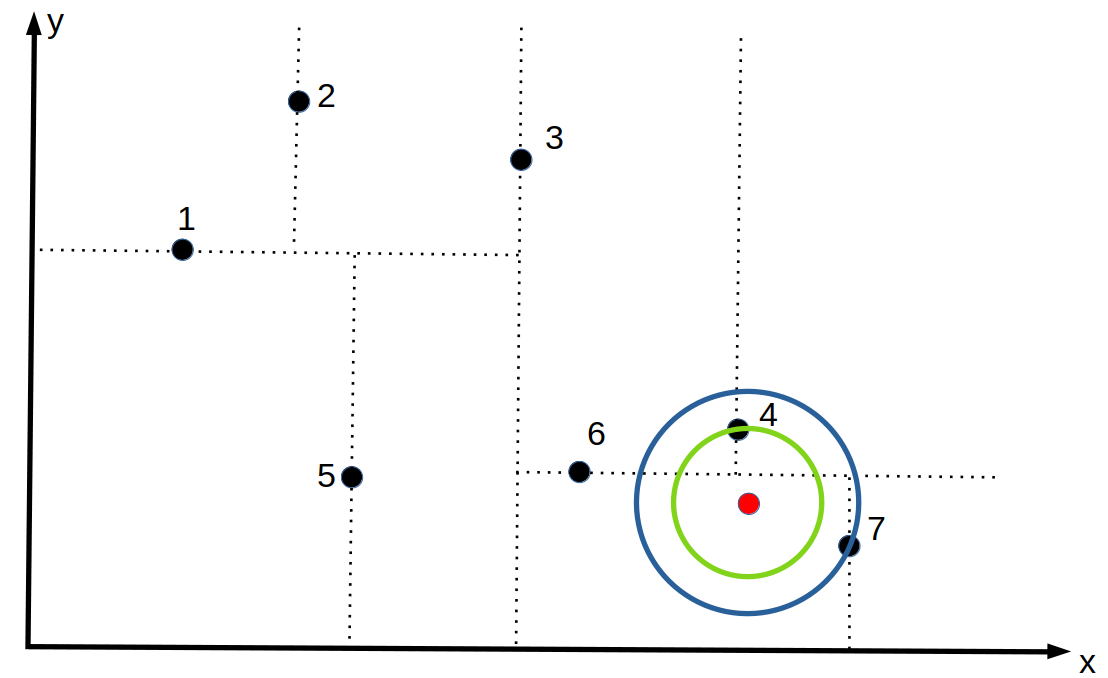
\includegraphics[height=6cm]{Developpements/arbre kdim/n+1_points.png}}
\raisebox{-0.5\height}{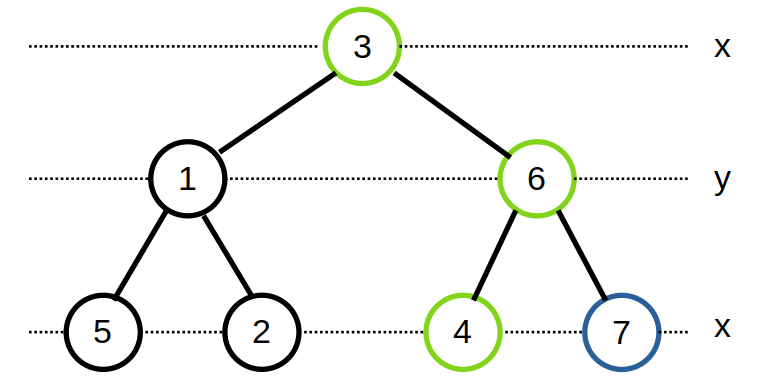
\includegraphics[height=4cm]{Developpements/arbre kdim/arbre_2.png}}

\section*{Complexité}

Construction de l'arbre : $C(n) = C(\left\lceil(n-1)/2\right\rceil ) + C(\left\lfloor(n-1)/2\right\rfloor ) + Mediane(n)$\\
Donc si la médiane est fait en temps linéaire : $C(n) = O(n\log(n))$\\

Pour la recherche : \begin{itemize}
	\item dans le pire des cas : $O(kn)$
	\item dans le meilleur des cas : $O(k\log n)$
	\item dans le cas moyen : $O(k\log n)$ avec un adversaire
\end{itemize}